% LuaLaTeX

\documentclass[a4paper, twoside, 12pt]{article}
\usepackage[latin]{babel}
%\usepackage[landscape, left=3cm, right=1.5cm, top=2cm, bottom=1cm]{geometry} % okraje stranky
%\usepackage[landscape, a4paper, mag=1166, truedimen, left=2cm, right=1.5cm, top=1.6cm, bottom=0.95cm]{geometry} % okraje stranky
\usepackage[landscape, a4paper, mag=1400, truedimen, left=0.5cm, right=0.5cm, top=0.5cm, bottom=0.5cm]{geometry} % okraje stranky

\usepackage{fontspec}
\setmainfont[FeatureFile={junicode.fea}, Ligatures={Common, TeX}, RawFeature=+fixi]{Junicode}
%\setmainfont{Junicode}

% shortcut for Junicode without ligatures (for the Czech texts)
\newfontfamily\nlfont[FeatureFile={junicode.fea}, Ligatures={Common, TeX}, RawFeature=+fixi]{Junicode}

\usepackage{multicol}
\usepackage{color}
\usepackage{lettrine}
\usepackage{fancyhdr}

% usual packages loading:
\usepackage{luatextra}
\usepackage{graphicx} % support the \includegraphics command and options
\usepackage{gregoriotex} % for gregorio score inclusion
\usepackage{gregoriosyms}
\usepackage{wrapfig} % figures wrapped by the text
\usepackage{parcolumns}
\usepackage[contents={},opacity=1,scale=1,color=black]{background}
\usepackage{tikzpagenodes}
\usepackage{calc}
\usepackage{longtable}
\usetikzlibrary{calc}

\setlength{\headheight}{14.5pt}

% Commands used to produce a typical "Conventus" booklet

\newenvironment{titulusOfficii}{\begin{center}}{\end{center}}
\newcommand{\dies}[1]{#1

}
\newcommand{\nomenFesti}[1]{\textbf{\Large #1}

}
\newcommand{\celebratio}[1]{#1

}

\newcommand{\hora}[1]{%
\vspace{0.5cm}{\large \textbf{#1}}

\fancyhead[LE]{\thepage\ / #1}
\fancyhead[RO]{#1 / \thepage}
\addcontentsline{toc}{subsection}{#1}
}

% larger unit than a hora
\newcommand{\divisio}[1]{%
\begin{center}
{\Large \textsc{#1}}
\end{center}
\fancyhead[CO,CE]{#1}
\addcontentsline{toc}{section}{#1}
}

% a part of a hora, larger than pars
\newcommand{\subhora}[1]{
\begin{center}
{\large \textit{#1}}
\end{center}
%\fancyhead[CO,CE]{#1}
\addcontentsline{toc}{subsubsection}{#1}
}

% rubricated inline text
\newcommand{\rubricatum}[1]{\textit{#1}}

% standalone rubric
\newcommand{\rubrica}[1]{\vspace{3mm}\rubricatum{#1}}

\newcommand{\notitia}[1]{\textcolor{red}{#1}}

\newcommand{\scriptura}[1]{\hfill \small\textit{#1}}

\newcommand{\translatioCantus}[1]{\vspace{1mm}%
{\noindent\footnotesize \nlfont{#1}}}

% pruznejsi varianta nasledujiciho - umoznuje nastavit sirku sloupce
% s prekladem
\newcommand{\psalmusEtTranslatioB}[3]{
  \vspace{0.5cm}
  \begin{parcolumns}[colwidths={2=#3}, nofirstindent=true]{2}
    \colchunk{
      \input{#1}
    }

    \colchunk{
      \vspace{-0.5cm}
      {\footnotesize \nlfont
        \input{#2}
      }
    }
  \end{parcolumns}
}

\newcommand{\psalmusEtTranslatio}[2]{
  \psalmusEtTranslatioB{#1}{#2}{8.5cm}
}


\newcommand{\canticumMagnificatEtTranslatio}[1]{
  \psalmusEtTranslatioB{#1}{temporalia/extra-adventum-vespers/magnificat-boh.tex}{12cm}
}
\newcommand{\canticumBenedictusEtTranslatio}[1]{
  \psalmusEtTranslatioB{#1}{temporalia/extra-adventum-laudes/benedictus-boh.tex}{10.5cm}
}

% volne misto nad antifonami, kam si zpevaci dokresli neumy
\newcommand{\hicSuntNeumae}{\vspace{0.5cm}}

% prepinani mista mezi notovymi osnovami: pro neumovane a neneumovane zpevy
\newcommand{\cantusCumNeumis}{
  \setgrefactor{17}
  \global\advance\grespaceabovelines by 5mm%
}
\newcommand{\cantusSineNeumas}{
  \setgrefactor{17}
  \global\advance\grespaceabovelines by -5mm%
}

% znaky k umisteni nad inicialu zpevu
\newcommand{\superInitialam}[1]{\gresetfirstlineaboveinitial{\small {\textbf{#1}}}{\small {\textbf{#1}}}}

% pars officii, i.e. "oratio", ...
\newcommand{\pars}[1]{\textbf{#1}}

\newenvironment{psalmus}{
  \setlength{\parindent}{0pt}
  \setlength{\parskip}{5pt}
}{
  \setlength{\parindent}{10pt}
  \setlength{\parskip}{10pt}
}

%%%% Prejmenovat na latinske:
\newcommand{\nadpisZalmu}[1]{
  \hspace{2cm}\textbf{#1}\vspace{2mm}%
  \nopagebreak%

}

% mode, score, translation
\newcommand{\antiphona}[3]{%
\hicSuntNeumae
\superInitialam{#1}
\includescore{#2}

#3
}
 % Often used macros
%%%% Preklady jednotlivych zpevu (nektere se opakuji, a je dobre mit je
% vsechny na jedne hromade)

\newcommand{\trOratioAnteOfficium}{\translatioCantus{Otevři, Pane, má ústa, abych chválil tvé svaté jméno.
Očisti mé srdce od všech marnivých, zvrácených a~jiných myšlenek, osvěť rozum, rozněť cit,
abych mohl důstojně, soustředěně a~zbožně recitovat a~vysloužil si být
vyslyšen před tváří tvé velebnosti. Skrze Krista…}}

\newcommand{\trOratioPostOfficium}{\translatioCantus{\textit{Následující modlitbu
opatřil pro ty, kdo ji zbožně vyřknou po hodinkách, zesnulý papež Lev X.
odpustky za hříchy vzniklé při konání hodinek z~lidské křehkosti. Říká se
vkleče.}
Svatosvaté a~nerozdílné Trojici, ukřižovanému lidství našeho Pána Ježíše
Krista, přeblažené a~přeslavné plodné neporušenosti vždy Panny Marie
i~souhrnu všech svatých buď ode všeho stvoření věčná chvála, čest a~sláva, nám
pak buď dáno odpuštění všech hříchů, po nekonečné věky věků. Amen.}}

% HOURS ---

\newcommand{\trAntI}{\translatioCantus{Jasné narození slavné Panny Marie,
z pokolení (dosl. ze semene) Abrahámova, vzešlé z kmene Judova, z rodu Davidova.}}
\newcommand{\trAntII}{\translatioCantus{Dnes je Narození svaté Panny 
Marie, jejíž předrahý život osvěcuje všechny církve.}}

\newcommand{\trAntIII}{\translatioCantus{Maria, jež vzešla 
z královského rodu, září; myslí i duchem ji zbožně prosíme, aby 
nám pomáhala svými přímluvami.}}

\newcommand{\trAntIV}{\translatioCantus{Srdcem i duchem pějme Kristu 
k slávě o této svaté slavnosti vznešené Rodičky Boží Marie.}}

\newcommand{\trAntV}{\translatioCantus{Příjemně \notitia{?} 
oslavujme Narození blahoslavené Marie,
aby se ona za nás přimlouvala u Pána Ježíše Krista.}}

\newcommand{\trCapituli}{\translatioCantus{Před věky, na počátku mě stvořil, potrvám věčně. Ve svatém Stanu jsem před ním konala službu.}}

\newcommand{\trRespVesp}{\translatioCantus{Buď zdráva, Maria,
plná milosti: \grestar{} Pán s tebou. \Vbardot{} Požehnaná jsi mezi ženami,
a požehnaný plod života (ve smyslu lůna, břicha) tvého.}}

\newcommand{\trVersus}{\translatioCantus{\Vbardot{} Dnes je Narození svaté Panny Marie. \Rbardot{} Jejíž předrahý život osvěcuje všechny církve.}}

\newcommand{\trAntMagnificatI}{\translatioCantus{Konejme památku
veledůstojného narození slavné Panny Marie,
jíž se dostalo mateřské důstojnosti bez ztráty panenské cudnosti.}}

% Tento preklad je vice nez nejisty a ani alternativy, ktere jsem
% videl, me nepresvedcily...
\newcommand{\trAntBenedictus}{\translatioCantus{Slavnostně slavme 
dnešní narození Marie, vždy Panny a Rodičky Boží: v něm se objevuje
vysokost trůnu (totiž Marie, trůnu Božího Syna), aleluja.}}

\newcommand{\trAntMagnificatII}{\translatioCantus{Tvé narození,
Bohorodičko Panno, vyhlásilo radost celému světu:
z tebe totiž vzešlo Slunce spravedlnosti, Kristus, náš Bůh:
jenž zrušil kletbu a dal nám požehnání: přemohl smrt a dal nám život věčný.}}

\newcommand{\trOrationis}{\translatioCantus{Prosíme tě, Bože, 
uděl svým služebníkům dar nebeské milosti,
aby těm, jimž slehnutím blahoslavené Panny vyvstal počátek spásy, 
slavnost k poctě jejího narození přinesla
rozhojnění pokoje.
Skrze tvého Syna, našeho Pána Ježíše Krista, který s tebou žije a kraluje,
Bůh, v jednotě Ducha svatého po všechny věky věků.}}

\newcommand{\trFideliumAnimae}{\translatioCantus{\Vbardot{} Duše věrných ať pro
milosrdenství Boží odpočívají v~pokoji. \Rbardot{} Amen.}}

% Completorium

\newcommand{\trJubeDomne}{\translatioCantus{Rač, pane, požehnat.}}

\newcommand{\trComplBenedictio}{\translatioCantus{Pokojnou noc a~svatou smrt
nechť nám dopřeje všemohoucí Pán. \Rbardot{} Amen.}}

\newcommand{\trComplLectioBr}{\translatioCantus{Buďte střízliví, bděte.
Váš protivník Ďábel obchází jako lev řvoucí a~hledá, koho by pohltil.
Postavte se proti němu pevní ve víře.  Ale ty, Pane, smiluj se nad námi.
\Rbardot{} Bohu díky.}}

\newcommand{\trComplAntI}{\translatioCantus{Rač se smilovati nade mnou,
Hospodine, a vyslyš mou modlitbu.}}

\newcommand{\trComplCapituli}{\translatioCantus{Jsi přece, Hospodine,
uprostřed nás a~jmenujeme se po tobě.  Neopouštěj nás, Pane, náš Bože.}}

\newcommand{\trRespCompl}{\translatioCantus{Do tvých rukou, Pane, \grestar{}
poroučím svého ducha. \Vbardot{} Ty mne zachráníš, Pane, Bože věrný.}}

\newcommand{\trComplVersus}{\translatioCantus{\Vbardot{} Střez mne jako zřítelnici oka,
aleluja. \Rbardot{} Ve stínu svých křídel uschovej mne, aleluja.}}

\newcommand{\trAntSalvaNos}{\translatioCantus{Ochraňuj nás, Pane, když
bdíme, a~buď s~námi, když spíme, ať bdíme s~Kristem a~odpočíváme v~pokoji.}}

\newcommand{\trComplOrationis}{\translatioCantus{Zavítej, prosíme, Pane, sem
do našeho příbytku a~daleko od něj zažeň všechny úklady nepřítele. Ať tu
bydlí tví svatí andělé a~tvoje požehnání buď nad ním stále. Skrze…}}

\newcommand{\trSalveRegina}{\translatioCantus{Zdrávas Královno, matko
milosrdenství, živote, sladkosti a naděje naše, buď zdráva!
K tobě voláme, vyhnaní synové Evy,
k tobě vzdycháme, lkajíce a plačíce
v tomto slzavém údolí.
A proto, orodovnice naše,
obrať k nám své milosrdné oči
a Ježíše, požehnaný plod života svého,
nám po tomto putování ukaž,
ó milostivá, ó přívětivá,
ó přesladká, Panno Maria!}}

\newcommand{\trOraProNobis}{\translatioCantus{\Vbardot{} 
Oroduj za nás, svatá Boží Rodičko,
\Rbardot{} aby nám Kristus dal účast na svých zaslíbeních.}}

% Matutinum

\newcommand{\trMatInvitatorium}{\translatioCantus{}}

\newcommand{\trMatVeniteA}{\translatioCantus{Pojďte, chvalme s~radostí Pána,
s~jásotem slavme Boha, svou spásu; předstupme před tvář jeho s~díky, písně plesu pějme jemu.}}

\newcommand{\trMatVeniteB}{\translatioCantus{Neboť Bůh veliký jest Hospodin, a~král nade všecky bohy.
Jsouť v~jeho ruce všecky hlubiny země, temena hor jsou majetek jeho.}}

\newcommand{\trMatVeniteC}{\translatioCantus{Jehoť jest moře, neb on je učinil; i~souš
je dílo jeho rukou. Pojďme, klanějme se, padněme, klekněme před Pánem, svým
tvůrcem. Jeť on Pán, náš Bůh, a~my jsme lid, jejž on vodí a~ovce, jež pase.}}

\newcommand{\trMatVeniteD}{\translatioCantus{Kéž byste poslechli dnes hlasu jeho:
,,Nezatvrzujte svých srdcí jak v~Hádce, jak v~Pokušení na poušti, kde vaši otcové pokoušeli mne,
zkoušeli mne, ač vídali skutky mé.``}}

\newcommand{\trMatVeniteE}{\translatioCantus{Čtyřicet roků mrzel jsem se na to pokolení
a~řekl jsem: ,,Lid je to myslí stále bloudící``! Oni však nechtěli znáti mé cesty, takže jsem
přisáhl ve svém hněvu: ,,Nedojdou odpočinku mého!\mbox{}``}}

\newcommand{\trMatAntI}{\translatioCantus{}}

\newcommand{\trMatAntII}{\translatioCantus{}}

\newcommand{\trMatAntIII}{\translatioCantus{}}

\newcommand{\trMatVersusI}{\translatioCantus{}}

\newcommand{\trMatAbsolutioI}{\translatioCantus{Vyslyš Pane Ježíši Kriste
prosby svých služebníků \gredagger{} a~smiluj se nad námi, \grestar{} jenž
s~Otcem a~Duchem…}}

\newcommand{\trMatBenedictioI}{\translatioCantus{Rač, pane, požehnat.
Věčný Otec nám stále žehnej. \Rbardot{} Amen.}}

\newcommand{\trMatLecI}{\translatioCantus{Kéž by mě zulíbal polibky svých úst. 
Tvé milování je nad víno lahodnější;
vybraně voní tvé voňavky;
rozlévající se olej je tvé jméno,
proto tě dívky milují.
Strhni mě za sebou, poběžme!
Král mě uvedl do svých komnat;
budeš nám radostí a jásotem.
Víc než víno oslavíme tvé milování;
věru po právu jsi milován!
Snědá jsem, a přece krásná, jeruzalémské dcery,
jako stany kedarské,
jako šalmské závěsy.
}}

\newcommand{\trMatRespI}{\translatioCantus{}}

\newcommand{\trMatBenedictioII}{\translatioCantus{Rač, pane, požehnat.
Jednorozený Boží Syn nám žehnej \grestar{} a nám pomáhej. \Rbardot{} Amen.}}

\newcommand{\trMatLecII}{\translatioCantus{Nehleďte na mou osmahlou pleť:
to mě slunce ožehlo.
Synové mé matky se na mne rozzlobili,
poslali mě hlídat vinice.
A svou vinici, tu jsem nehlídala!
Pověz mi tedy, ty, jehož miluje mé srdce:
kam zavedeš své stádo pást,
kde ho necháš za poledne odpočívat?
Abych už nebloudila jako tulačka
poblíž stád druhů tvých.
Nevíš-li to, nejrásnější z žen,
jdi po stopách stáda
a kůzlata svá zaveď, ať se pasou
poblíž obydlí pastýřů.
Ke své klisně zapřažené do vozu faraonova
tebe, mé milá, přirovnávám.
Stále krásné jsou tvé líce s náušnicemi
i tvé hrdlo v náhrdelnících.}}

\newcommand{\trMatRespII}{\translatioCantus{}}

\newcommand{\trMatBenedictioIII}{\translatioCantus{Rač, pane, požehnat.
Milost Ducha Svatého ať osvítí nám smysly \grestar{} i srdce. \Rbardot{} Amen.}}

\newcommand{\trMatLecIII}{\translatioCantus{Zhotovíme ti zlaté náušnice
a kuličky ze stříbra.
Když král stoluje,
vydechuje můj nard svou vůni.
Můj milý je polštářek s myrhou,
jenž mi odpočívá mezi ňadry.
Můj milý je hrozen šáchoru
ve vinicích v Engadi.
Jak jsi krásná, milá moje,
jak jsi krásná!
Tvé oči jsou holubice.
Jak jsi krásný, můj milý,
jak líbezný!
Naše lože je samá zeleň.
Trámoví našeho domu je z cedru,
naše ostění z cypřiše.}}

\newcommand{\trMatRespIII}{\translatioCantus{}}

\newcommand{\trMatAntIV}{\translatioCantus{}}

\newcommand{\trMatAntV}{\translatioCantus{}}

\newcommand{\trMatAntVI}{\translatioCantus{}}

\newcommand{\trMatVersusII}{\translatioCantus{}}

\newcommand{\trMatAbsolutioII}{\translatioCantus{
Tvá milost a laskavost nechť nám pomáhá, jenž žiješ a vládneš s Otcem a Svatým Duchem na věky věků.}}

\newcommand{\trMatBenedictioIV}{\translatioCantus{Rač, pane, požehnat.
Bůh Otec všemohoucí, \grestar{} buď k nám milostivý a odpouštějící. \Rbardot{} Amen.}}

\newcommand{\trMatLecIV}{\translatioCantus{}}

\newcommand{\trMatRespIV}{\translatioCantus{}}

\newcommand{\trMatBenedictioV}{\translatioCantus{}}

\newcommand{\trMatLecV}{\translatioCantus{}}

\newcommand{\trMatRespV}{\translatioCantus{}}

\newcommand{\trMatBenedictioVI}{\translatioCantus{Rač, pane, požehnat.
Bůh rozněť v nás oheň své lásky. \Rbardot{} Amen.}}

\newcommand{\trMatLecVI}{\translatioCantus{}}

\newcommand{\trMatRespVI}{\translatioCantus{}}

\newcommand{\trMatAntVII}{\translatioCantus{}}

\newcommand{\trMatAntVIII}{\translatioCantus{}}

\newcommand{\trMatAntIX}{\translatioCantus{}}

\newcommand{\trMatVersusIII}{\translatioCantus{}}

\newcommand{\trMatAbsolutioIII}{\translatioCantus{Z okovů našich hříchů,
\grestar{} vysvoboď nás všemohoucí a milosrdný Pán. \Rbardot{} Amen.}}

\newcommand{\trMatBenedictioVII}{\translatioCantus{Rač, pane, požehnat.
Čtení evangelia nechť je nám \grestar{} spásou a ochranou. \Rbardot{} Amen.}}

\newcommand{\trMatLecVIIa}{\translatioCantus{
  Rodokmen Ježíše Krista, syna Davidova, syna Abrahámova:
  Abrahám zplodil Izáka,
  Izák zplodil Jakuba.}}

\newcommand{\trMatLecVIIb}{\translatioCantus{}}

\newcommand{\trMatRespVII}{\translatioCantus{}}

\newcommand{\trMatBenedictioVIII}{\translatioCantus{Rač, pane, požehnat.
\Rbardot{} Amen.}}

\newcommand{\trMatLecVIII}{\translatioCantus{}}

\newcommand{\trMatRespVIII}{\translatioCantus{}}

\newcommand{\trMatBenedictioIX}{\translatioCantus{Rač, pane, požehnat.
Do společnosti občanů nebes \grestar{} ať nás dovede král andělů.
\Rbardot{} Amen.}}

\newcommand{\trMatLecIX}{\translatioCantus{}}

% from the Czech Liturgia horarum
\newcommand{\trTeDeum}{\begin{translatioMulticol}{3}

Bože, tebe chválíme, 
tebe, Pane, velebíme.

Tebe, věčný Otče, 
oslavuje celá země.

Všichni andělé, 
cherubové i~serafové,

všechny mocné nebeské zástupy 
bez ustání volají:

Svatý, Svatý, Svatý, 
Pán, Bůh zástupů.

Plná jsou nebesa i~země 
tvé vznešené slávy.

Oslavuje tě 
sbor tvých apoštolů,

chválí tě 
velký počet proroků,

vydává o~tobě svědectví 
zástup mučedníků;

a~po celém světě 
vyznává tě tvá církev:

neskonale velebný, 
všemohoucí Otče,

úctyhodný Synu Boží, 
pravý a~jediný,

božský Utěšiteli, 
Duchu svatý.

Kriste, Králi slávy, 
tys od věků Syn Boha Otce;

abys člověka vykoupil, 
stal ses člověkem a~narodil ses z~Panny;

zlomil jsi osten smrti 
a~otevřel věřícím nebe;

sedíš po Otcově pravici 
a~máš účast na jeho slávě.

Věříme, že přijdeš soudit, 

a~proto tě prosíme:
přispěj na pomoc svým služebníkům, 
vždyť jsi je vykoupil svou předrahou krví;

dej, ať se radují s~tvými svatými 
ve věčné slávě.

Zachraň, Pane, svůj lid, žehnej svému dědictví, 
veď ho a~stále pozvedej.

Každý den tě budeme velebit 
a~chválit tvé jméno po všechny věky.

Pomáhej nám i~dnes, 
ať se nedostaneme do područí hříchu.

Smiluj se nad námi, Pane, 
smiluj se nad námi.

Ať spočine na nás tvé milosrdenství, 
jak doufáme v~tebe.

Pane, k~tobě se utíkáme, 
ať nejsme zahanbeni na věky. 
\end{translatioMulticol}}

\newcommand{\trMatEvangelium}{\translatioCantus{
  Rodokmen Ježíše Krista, syna Davidova, syna Abrahámova:
  Abrahám zplodil Izáka,
  Izák zplodil Jakuba,
  Jakub zplodil Judu a jeho bratry,
  Juda zplodil Farese a Zaru z Tamary,
  Fares zplodil Esroma,
  Esrom zplodil Arama,
  Aram zplodil Aminadaba,
  Aminadab zplodil Naasona,
  Naason zplodil Salmona,
  Salmon zplodil Boaze z Rahaby,
  Boaz zplodil Jobeda z Rut,
  Jobed zplodil Jessea,
  Jesse zplodil krále Davida.
  David zplodil Šalomouna z Uriášovy ženy,
  Šalomoun zplodil Roboama,
  Roboam zplodil Abiu,
  Abia zplodil Asu,
  Asa zplodil Josafata,
  Josafat zplodil Jorama,
  Joram zplodil Oziáše,
  Oziáš zplodil Joatama,
  Joatam zplodil Achaze,
  Achaz zplodil Ezechiáše,
  Ezechiáš zplodil Manasesa,
  Manases zplodil Amona,
  Amon zplodil Josiáše,
  Josiáš zplodil Jechoniáše a jeho bratry;
  tehdy došlo k odvlečení do Babylonu.
  Po odvlečení do Babylonu:
  Jechoniáš zplodil Salatiela,
  Salatiel zplodil Zorobabela,
  Zorobabel zplodil Abiuda,
  Abiud zplodil Eljakima,
  Eljakim zplodil Azora,
  Ator zplodil Sadoka,
  Sadok zplodil Achima,
  Achim zplodil Eliuda,
  Eliud zplodil Eleazara,
  Eleatar zplodil Matana,
  Matan zplodil Jakuba,
  Jakub zplodil Josefa, manžela Marie,
  z níž se narodil Ježíš, který se nazývá Kristus.}}

\newcommand{\trTeDecetLaus}{\translatioCantus{Tobě chvála, Tobě zpěvy, Tobě
sláva, Bohu Otci i~Synu i~Svatému Duchu, na věky věků. \Rbardot{} Amen.}}

% MASS ---

\newcommand{\trIntroitus}{\translatioCantus{Radujme se všichni
v Pánu, slavíce svátek ke cti Panny Marie: z něj se radují andělé
a spoluchválí Božího Syna. \textit{\color{red}Žl.} Má ústa vydala dobré slovo,
přednáším svá díla králi.}}

\newcommand{\trGraduale}{\translatioCantus{Požehnaná a ctihodná jsi,
Panno Maria: nedotčená (co do panenství) jsi byla shledána matkou
Spasitele. \Vbardot{} Panno Boží Rodičko, ten, jehož nepojme ani celý svět,
se uzavřel do tvých útrob, když se stal člověkem.}}

\newcommand{\trAlleluia}{\translatioCantus{Aleluja. \Vbardot{} Skvělá slavnost
slavné Panny Marie, z pokolení (dosl. ze semene) Abrahámova, vzešlé z kmene 
Judova, z rodu Davidova.}}

\newcommand{\trOffertorium}{\translatioCantus{Blažená jsi, Panno Maria,
tys nosila Stvořitele všeho; porodila jsi toho, který tě utvořil,
a na věky zůstáváš Pannou.}}

\newcommand{\trCommunio}{\translatioCantus{Budou mě blahoslavit
všechna pokolení, protože mi učinil veliké věci ten, který je mocný.}}

% LITTLE HOURS ---

\newcommand{\trVersusTertia}{\translatioCantus{\Vbardot{} \Rbardot{}}}

\newcommand{\trCapituliEtSic}{\translatioCantus{
Tak jsem se usadila na Sionu a v milovaném městě jsem nalezla odpočinek,
v Jeruzalémě vykonávám svou moc.
Zakořenila jsem u lidu plného slývy, na panství Páně, v jeho dědictví.}}

\newcommand{\trVersusSexta}{\translatioCantus{\Vbardot{} \Rbardot{}}}

\newcommand{\trCapituliInPlateis}{\translatioCantus{
Na planině jako skořicovník a akant jsem vydávala vůni, jako vybraná myrha
jsem voněla.}}

\newcommand{\trVersusNona}{\translatioCantus{\Vbardot{} \Rbardot{}}}
 % Czech translations of the proper texts

\newcommand{\annusEditionis}{2020}

%%%% Vicekrat opakovane kousky

\newcommand{\anteOrationem}{
  \rubrica{Ante Orationem, cantatur a Superiore:}

  \pars{Supplicatio Litaniæ.}

  \cuminitiali{}{temporalia/supplicatiolitaniae.gtex}

  \pars{Oratio Dominica.}

  \cuminitiali{}{temporalia/oratiodominica.gtex}

  \rubrica{Deinde dicitur ab Hebdomadario:}

  \cuminitiali{}{temporalia/dominusvobiscum-solemnis.gtex}

  \rubrica{In choro monialium loco Dominus vobiscum dicitur:}

  \sineinitiali{temporalia/domineexaudi.gtex}
}

\setlength{\columnsep}{30pt} % prostor mezi sloupci

%%%%%%%%%%%%%%%%%%%%%%%%%%%%%%%%%%%%%%%%%%%%%%%%%%%%%%%%%%%%%%%%%%%%%%%%%%%%%%%%%%%%%%%%%%%%%%%%%%%%%%%%%%%%%
\begin{document}

% Here we set the space around the initial.
% Please report to http://home.gna.org/gregorio/gregoriotex/details for more details and options
\grechangedim{afterinitialshift}{2.2mm}{scalable}
\grechangedim{beforeinitialshift}{2.2mm}{scalable}
\grechangedim{interwordspacetext}{0.22 cm plus 0.15 cm minus 0.05 cm}{scalable}%
\grechangedim{annotationraise}{-0.2cm}{scalable}

% Here we set the initial font. Change 38 if you want a bigger initial.
% Emit the initials in red.
\grechangestyle{initial}{\color{red}\fontsize{38}{38}\selectfont}

\pagestyle{empty}

%%%% Titulni stranka
\begin{titulusOfficii}
\dies{Die 24. Maii.}
\nomenFesti{Beatæ Mariæ Virgo Mater Ecclesiæ.}
\end{titulusOfficii}

% graphic
%\vspace{1.5cm}
%\begin{center}
%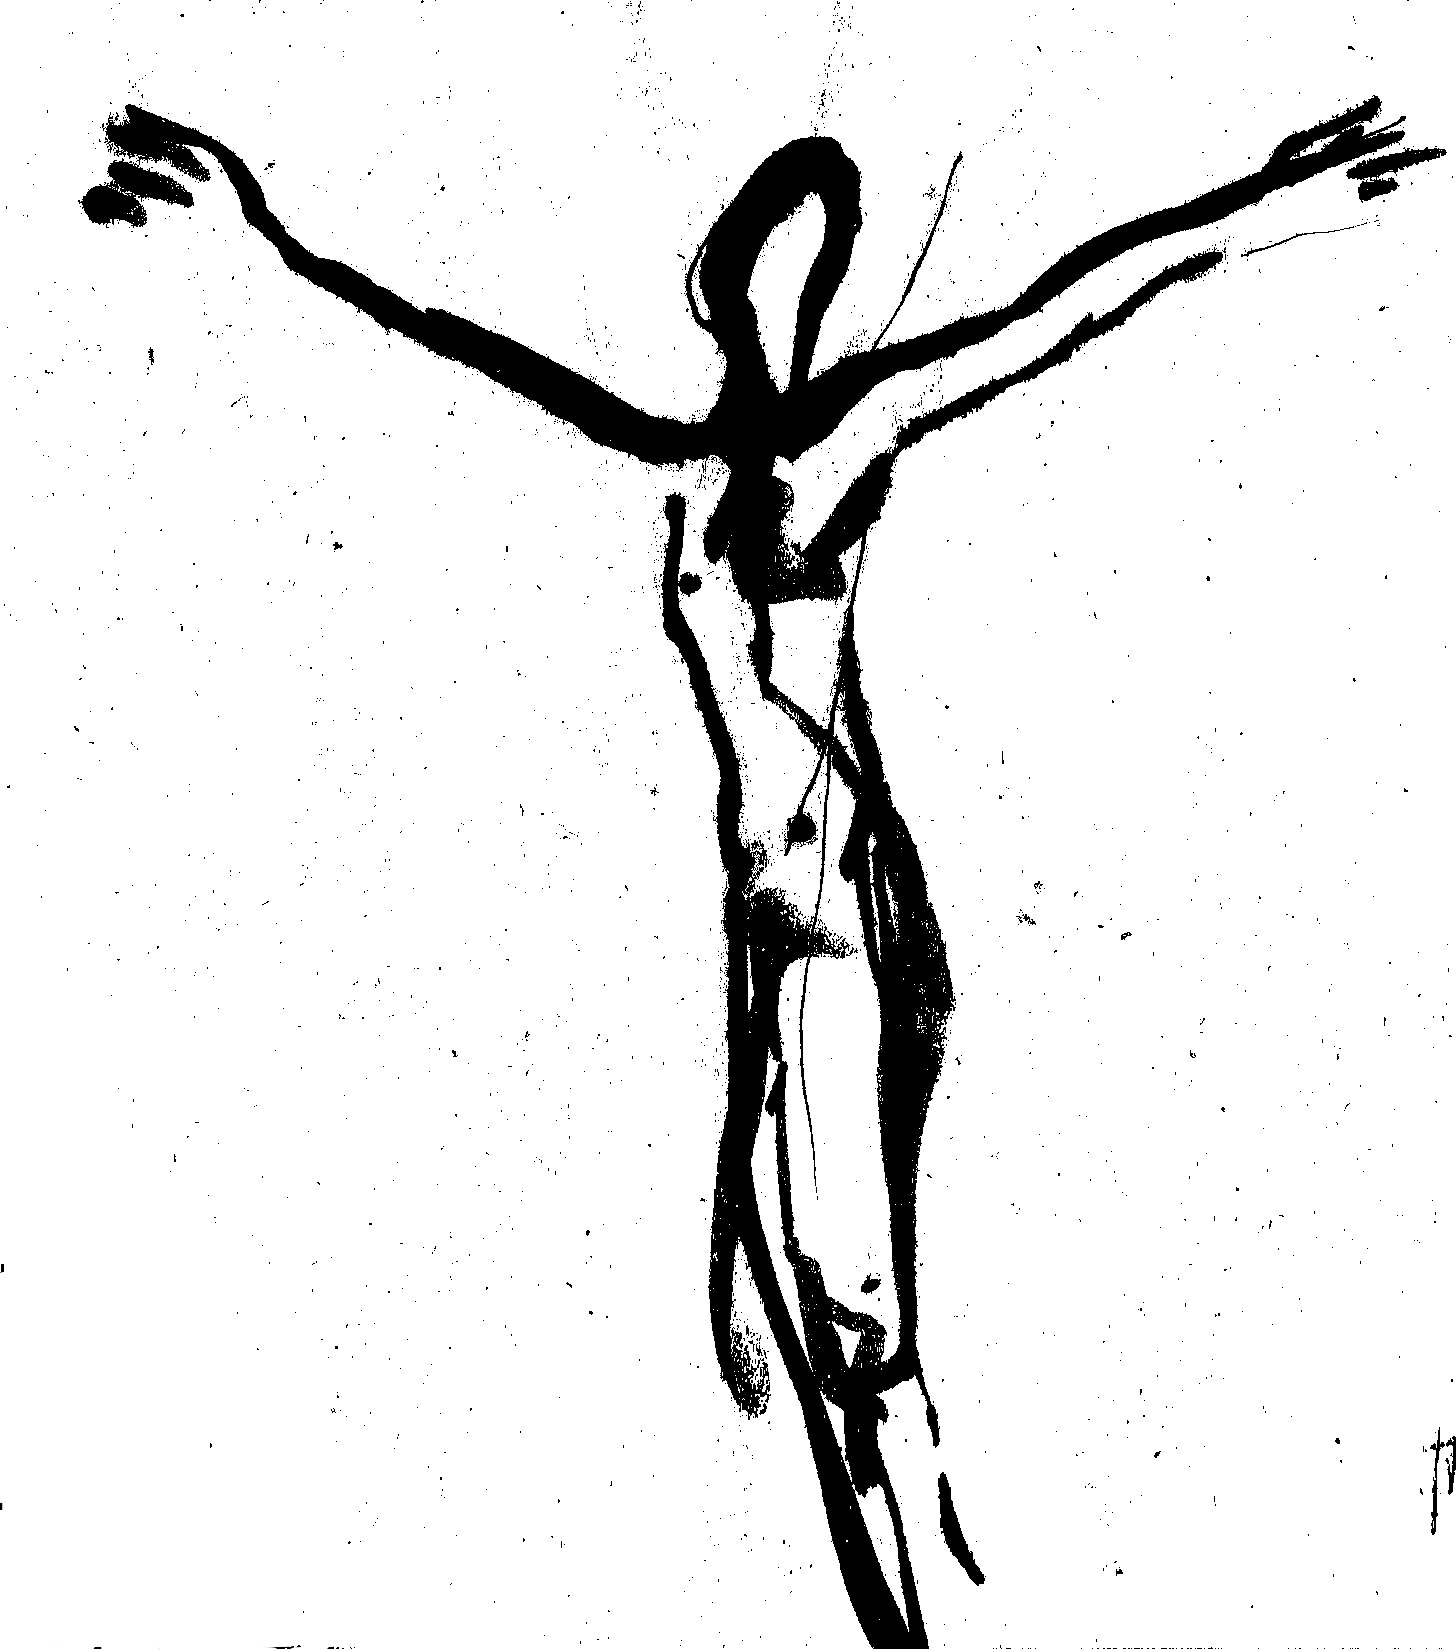
\includegraphics[height=8cm]{crux.jpg}
%\end{center}

\vfill

\begin{center}
%Ad usum et secundum consuetudines chori \guillemotright{}Conventus Choralis\guillemotleft.

%Editio Sancti Wolfgangi \annusEditionis
\end{center}

\pagebreak

\renewcommand{\headrulewidth}{0pt} % no horiz. rule at the header
\fancyhf{}
\pagestyle{fancy}

\cantusSineNeumas

\hora{Ad Matutinum.} %%%%%%%%%%%%%%%%%%%%%%%%%%%%%%%%%%%%%%%%%%%%%%%%%%%%%%%%%%
%\sideThumbs{Matutinum}

\vspace{2mm}

\cuminitiali{}{temporalia/dominelabiamea.gtex}

\vspace{2mm}

\pars{Invitatorium.} \scriptura{Lc. 1, 28; Psalmus 94}

\vspace{-6mm}

\antiphona{VII}{temporalia/inv-avemaria.gtex}

\vfill
\pagebreak

\pars{Hymnus.}

\vspace{-5mm}

{
\grechangedim{interwordspacetext}{0.30 cm plus 0.15 cm minus 0.05 cm}{scalable}%
\antiphona{II}{temporalia/hym-QuemTerra-alt.gtex}
\grechangedim{interwordspacetext}{0.22 cm plus 0.15 cm minus 0.05 cm}{scalable}%
}
\vfill
\pagebreak

%\subhora{In I. Nocturno}

\pars{Psalmus 1.} \scriptura{Lc. 1, 42; \textbf{H21}}

\vspace{-4mm}

\antiphona{II* a}{temporalia/ant-benedictatu.gtex}

%\trMatAntI

\scriptura{Psalmus 8.}

\initiumpsalmi{temporalia/ps8-initium-ii_-a.gtex}

%\psalmusEtTranslatioT{temporalia/ps8-comb.tex}{10cm}
\input{temporalia/ps8.tex} \Abardot{}

%\antiphona{}{temporalia/ant-benedictatu.gtex} % repeat the antiphon - new page

\vfill
\pagebreak

\pars{Psalmus 2.} \scriptura{Cf. Sir. 24, 20; \textbf{H115}}

\vspace{-4mm}

\antiphona{IV A}{temporalia/matant2.gtex}

%\trMatAntII

\scriptura{Psalmus 18.}

\initiumpsalmi{temporalia/ps18-initium-iv-A-auto.gtex}

%\psalmusEtTranslatioT{temporalia/ps18-comb.tex}{10cm}
\input{temporalia/ps18.tex}

\antiphona{}{temporalia/matant2.gtex} % repeat the antiphon - new page

\vfill
\pagebreak

\pars{Psalmus 3.} \scriptura{\textbf{H115}}

\vspace{-4mm}

\antiphona{IV c}{temporalia/ant-antethorum-FKP.gtex}

%\trMatAntIII

\scriptura{Psalmus 23.}

\initiumpsalmi{temporalia/ps23-initium-iv-c.gtex}

%\psalmusEtTranslatioT{temporalia/ps23-comb.tex}{10cm}
\input{temporalia/ps23.tex} \Abardot{}

\vfill
\pagebreak

\pars{Psalmus 4.} \scriptura{Ps. 44, 5; \textbf{H117}}

\vspace{-4mm}

\antiphona{VII c}{temporalia/matant4.gtex}

%\trMatAntIV

\scriptura{Psalmus 44.}

\initiumpsalmi{temporalia/ps44-initium-vii-c-auto.gtex}

%\psalmusEtTranslatioT{temporalia/ps44-comb.tex}{10cm}
\input{temporalia/ps44.tex}

\antiphona{}{temporalia/matant4.gtex} % repeat the antiphon - new page

\vfill
\pagebreak

\pars{Psalmus 5.} \scriptura{Ps. 45, 6; \textbf{H117}}

\vspace{-4mm}

\antiphona{VII c}{temporalia/matant5.gtex}

%\trMatAntV

\scriptura{Psalmus 45.}

\initiumpsalmi{temporalia/ps45-initium-vii-c-auto.gtex}

%\psalmusEtTranslatioT{temporalia/ps45-comb.tex}{10cm}
\input{temporalia/ps45.tex} \Abardot{}

%\antiphona{}{temporalia/matant5.gtex} % repeat the antiphon - new page

\vfill
\pagebreak

\pars{Psalmus 6.} \scriptura{Psalmus 86, 7; \textbf{H117}}

\vspace{-4mm}

\antiphona{VII c}{temporalia/matant6.gtex}

%\trMatAntVI

\scriptura{Psalmus 86.}

\initiumpsalmi{temporalia/ps86-initium-vii-c-auto.gtex}

%\psalmusEtTranslatioT{temporalia/ps86-comb.tex}{10cm}
\input{temporalia/ps86.tex} \Abardot{}

%\antiphona{}{temporalia/matant6.gtex} % repeat the antiphon - new page

\vfill
\pagebreak

\pars{Versus.} \scriptura{Ps. 44, 5}

\sineinitiali{temporalia/versus-specie.gtex}

\vspace{5mm}

\sineinitiali{temporalia/oratiodominica-mat.gtex}

\vspace{5mm}

\pars{Absolutio.}

\cuminitiali{}{temporalia/absolutio-exaudi.gtex}

%\trMatAbsolutioI

\vfill
\pagebreak

\cuminitiali{}{temporalia/benedictio-solemn-benedictione.gtex}

%\trMatBenedictioI

\vspace{7mm}

\pars{Lectio I.} \scriptura{Prov. 8, 12-17.34-36; 9, 1-5}

\noindent De Parábolis Salomónis.

\noindent Ego sapiéntia hábito in consílio et erudítis intérsum cogitatiónibus. Timor Dómini odit malum: arrogántiam, et supérbiam, et viam pravam, et os bilíngue detéstor. Meum est consílium et ǽquitas, mea est prudéntia, mea est fortitúdo. Per me reges regnant, et legum conditóres justa decérnunt; Per me príncipes ímperant, et poténtes decérnunt justítiam. Ego diligéntes me díligo; et qui mane vígilant ad me, invénient me. Mecum sunt divítiæ et glória, opes supérbæ et justítia. Mélior est enim fructus meus auro et lápide pretióso, et genímina mea argénto elécto. In viis justítiæ ámbulo, in médio semitárum judícii, Ut ditem diligéntes me et thesáuros eórum répleam. Dóminus possidébit me in inítio viárum suárum, ántequam quidquam fáceret a princípio. Ab ætérno ordináta sum et ex antíquis, ántequam terra fíeret. Nondum erant abýssi, et ego jam concépta eram; Necdum fontes aquárum erúperant, necdum montes gravi mole constíterant; ante colles ego parturiébar. Beátus homo qui audit me, et qui vígilat ad fores meas quotídie, et obsérvat ad postes óstii mei. Qui me invénerit, invéniet vitam, et háuriet salútem a Dómino; Qui autem in me peccáverit, lædet ánimam suam. Omnes, qui me odérunt, díligunt mortem. Sapiéntia ædificávit sibi domum, excídit colúmnas septem. Immolávit víctimas suas, míscuit vinum et propósuit mensam suam. Misit ancíllas suas ut vocárent ad arcem et ad mœ́nia civitátis: Si quis est párvulus, véniat ad me. Et insipiéntibus locúta est: Veníte, comédite panem meum, et bíbite vinum quod míscui vobis.

\noindent \Vbardot{} Tu autem, Dómine, miserére nobis.
\noindent \Rbardot{} Deo grátias.

\vfill
\pagebreak

\pars{Responsorium 1.} \scriptura{\Rbardot{} Ct. 6, 9 \Vbardot{} ibid. 3, 6; \textbf{H297}}

\vspace{-5mm}

\responsorium{IV}{temporalia/resp-quaeestista-CROCHU.gtex}{}

\vfill
\pagebreak

\cuminitiali{}{temporalia/benedictio-solemn-unigenitus.gtex}

%\trMatBenedictioII

\vspace{7mm}

\pars{Lectio II.} \scriptura{Sermo 25, 7-8: PL 46, 937-938}

\noindent Ex Sermónibus sancti Augustíni epíscopi.

\noindent Atténdite, óbsecro vos, quod ait Dóminus Christus, exténdens manum super discípulos suos: Hæc est mater mea et fratres mei; et qui fécerit voluntátem Patris mei, qui me misit, ipse mihi et frater et soror et mater est. Numquid non fecit voluntátem Patris Virgo María, quæ fide crédidit, fide concépit, elécta est de qua nobis salus inter hómines nascerétur, creáta est a Christo ántequam in illa Christus crearétur? Fecit, fecit plane voluntátem Patris sancta María, et ídeo plus est Maríæ discípulam fuísse Christi, quam matrem fuísse Christi; plus est felícius discípulam fuísse Christi quam matrem fuísse Christi. Ideo María beáta erat, quia et ántequam páreret magístrum, in útero portávit. Vide si non est quod dico. Transeúnte Dómino cum turbis sequéntibus et mirácula faciénte divína, ait quædam múlier: Felix venter, qui te portávit. Beátus venter, qui te portávit. Et Dóminus, ut non felícitas in carne quærerétur, quid respóndit? Immo beáti qui áudiunt verbum Dei et custódiunt. Inde ergo et María beáta, quia audívit verbum Dei et custodívit; plus mente custodívit veritátem quam útero carnem. Véritas Christus, caro Christus: véritas Christus in mente Maríæ, caro Christus in ventre Maríæ; plus est quod est in mente, quam quod portátur in ventre.

\noindent \Vbardot{} Tu autem, Dómine, miserére nobis.
\noindent \Rbardot{} Deo grátias.

\vfill
\pagebreak

\pars{Responsorium 2.} \scriptura{\Rbardot{} Ps. 44, 12 \Vbardot{} ibid., 5; \textbf{H298}}

\vspace{-5mm}

\responsorium{II}{temporalia/resp-venielectamea-CROCHU.gtex}{}

\vfill
\pagebreak

\cuminitiali{}{temporalia/benedictio-solemn-spiritus.gtex}

%\trMatBenedictioIII

\vspace{7mm}

\pars{Lectio III.}

\noindent Sancta María, beáta María, sed mélior est Ecclésia quam Virgo María. Quare? Quia María pórtio est Ecclésiæ, sanctum membrum, excéllens membrum, superéminens membrum, sed tamen totíus córporis membrum. Si totíus córporis, plus est profécto corpus quam membrum. Caput Dóminus et totus Christus caput et corpus. Quid dicam? Divínum caput habémus, Deum caput habémus. Ergo, caríssimi, vos atténdite: et vos membra Christi estis, et vos corpus Christi estis. Atténdite quómodo sitis, quod ait: Ecce mater mea et fratres mei. Quómodo éritis mater Christi? Et quicúmque audit, et quicúmque facit voluntátem Patris mei qui in cælis est, ipse meus frater et soror et mater est. Puta, fratres intéllego, soróres intéllego: una est enim heréditas, et ídeo Christi misericórdia, qui cum esset únicus, nóluit esse solus, vóluit nos esse Patri herédes, sibi coherédes.

\noindent \Vbardot{} Tu autem, Dómine, miserére nobis.
\noindent \Rbardot{} Deo grátias.

\vfill
\pagebreak

\pars{Responsorium 3.} \scriptura{\Vbardot{} Ps. 44, 5; \textbf{H298}}

\vspace{-5mm}

\responsorium{II}{temporalia/resp-istaestspeciosa.gtex}{}

\vfill
\pagebreak

\sineinitiali{temporalia/domineexaudi.gtex}

\vfill

\pars{Oratio.}

\cuminitiali{}{temporalia/oratio.gtex}
%\trOrationis

\vfill

\noindent \Vbardot{} Dómine, exáudi oratiónem meam.
\Rbardot{} Et clamor meus ad te véniat.

\vfill

% Nocturnale Romanum 2002, p. LXXVI Benedicamus Domino seems to match
% the one from Solemn Laudes.
\cuminitiali{V}{temporalia/benedicamus-solemnis-laud.gtex}

\vfill

\noindent \Vbardot{} Fidélium ánimæ per misericórdiam Dei requiéscant in pace.
\Rbardot{} Amen.

%\trFideliumAnimae

\vfill
\pagebreak

\hora{Ad Laudes.} %%%%%%%%%%%%%%%%%%%%%%%%%%%%%%%%%%%%%%%%%%%%%%%%%%%%%%%%%%

\pars{ } \scriptura{ }
\cantusSineNeumas
%\sideThumbs{Laudes}

% Psalmi festivi (AM33, pg. 721):
% 66 // 92, 99, 62, Dan3, 148+149+150

%\vspace{1cm}
\cuminitiali{}{temporalia/deusinadiutorium-alter.gtex}
%\vspace{1cm}

\cantusSineNeumas

\vspace{5mm}

\pars{Hymnus.}

\cuminitiali{II}{temporalia/hym-OGloriosaFemina.gtex}
%\input{cantus/amon33/hym-OGloriosaFemina-bohtext.tex}

\vfill
\pagebreak

\pars{Psalmus 1.} \scriptura{Idt. 13, 23; \textbf{H299}}

\vspace{-4mm}

\antiphona{VII c2}{temporalia/ant-benedictafilia.gtex}

%\vspace{-2mm}

%\trAntIII

\scriptura{Ps. 62.}

\initiumpsalmi{temporalia/ps62-initium-vii-c2-auto.gtex}

%\vspace{-6mm}

%\psalmusEtTranslatioT{temporalia/ps62-comb.tex}{10cm}
\input{temporalia/ps62.tex} \Abardot{}

\vfill
\pagebreak

\pars{Psalmus 2.}

\vspace{-4mm}

\antiphona{VIII c}{temporalia/ant-tugloriosajerusalem.gtex}

%\vspace{-2mm}

%\trAntIV

\scriptura{Canticum trium puerorum, Dan. 3, 57-88 et 56}

\vspace{-2mm}

\initiumpsalmi{temporalia/dan3-initium-viii-c-auto.gtex}

%\psalmusEtTranslatioT{temporalia/dan3-comb.tex}{10cm}
\input{temporalia/dan3.tex}

\rubrica{Hic non dicitur Gloria Patri, neque Amen.}
\vspace{1cm}

\antiphona{}{temporalia/ant-tugloriosajerusalem.gtex} % repeat the antiphon - new page

\vfill
\pagebreak

\pars{Psalmus 3.} \scriptura{Ct. 6, 8}

\vspace{-4mm}

\antiphona{VI F}{temporalia/ant-viderunteamfiliae.gtex}

%\vspace{-2mm}

%\trAntV

\scriptura{Ps. 149}

\initiumpsalmi{temporalia/ps149-initium-vi-F-auto.gtex}

%\psalmusEtTranslatioT{temporalia/ps149-comb.tex}{10cm}
\input{temporalia/ps149.tex}

\begin{psalmus}

Glória Pa\-tri \emph{et }\textbf{Fí}\-lio,~\grestar{} 
et Spirí\emph{\-tui }\textbf{Sanc}\-to.

Sicut erat in princípio, et nunc\emph{ et }\textbf{sem}\-per,~\grestar{} 
et in sǽcula sæcu\emph{ló\-rum. }\textbf{A}\-men.
\end{psalmus} \Abardot{}

\vfill
\pagebreak

\cantusSineNeumas

\pars{Lectio brevis.} \scriptura{Cf. Is. 61, 10}

\noindent Gaudens gaudébo in Dómino, et exsultábit ánima mea in Deo meo, quia índuit me vestiméntis salútis et induménto iustítiæ circúmdedit me, quasi sponsam ornátam monílibus suis.

\vfill
\pars{Responsorium breve.} \scriptura{Ps. 44, 3}

\antiphona{VI}{temporalia/resp-diffusaest.gtex}

%\trRespVesp

\vfill
\pagebreak

\pars{Canticum Zachariæ.}

\vspace{-4mm}

\antiphona{I f}{temporalia/ant-paradisiportaperevam.gtex}

%\trAntBenedictus

%\vspace{-2mm}

\scriptura{Lc. 1, 68-79}

%\vspace{-2mm}

\initiumpsalmi{temporalia/benedictus-initium-isoll-f-auto.gtex}

%\vspace{-1.5mm}

%\psalmusEtTranslatioT{temporalia/benedictus-comb.tex}{10cm}
\input{temporalia/benedictus.tex} \Abardot{}

\vfill
\pagebreak

\cantusSineNeumas

\pars{Preces.}

\sineinitiali{}{temporalia/tonusprecum.gtex}

\noindent Salvatórem nostrum celebrántes, qui ex María Vírgine nasci dignátus est, \gredagger{} exorémus dicéntes:

\Rbardot{} Intercédat pro nobis mater tua, Dómine.

\noindent O sol iustítiæ, quem Immaculáta Virgo ut lucens auróra præcéssit, \gredagger{} tríbue ut in lúmine visitatiónis tuæ semper ambulémus.

\Rbardot{} Intercédat pro nobis mater tua, Dómine.

\noindent Verbum ætérnum, quod Maríam habitatiónis tuæ arcam incorruptíbilem elegísti, \gredagger{} líbera nos a corruptióne peccáti.

\Rbardot{} Intercédat pro nobis mater tua, Dómine.

\noindent Salvátor noster, qui iuxta crucem matrem tuam habuísti, \gredagger{} præsta ut, ipsa intercedénte, communicántes tuis passiónibus gaudeámus.

\Rbardot{} Intercédat pro nobis mater tua, Dómine.

\noindent Benigníssime Iesu, qui pendens in cruce, Maríam Ioánni matrem dedísti, \gredagger{} da nobis ita vívere ut eius fílii agnoscámur.

\Rbardot{} Intercédat pro nobis mater tua, Dómine.

\vfill

\pars{Oratio Dominica.}

\cuminitiali{}{temporalia/oratiodominicaalt.gtex}

\vfill
\pagebreak

\rubrica{vel:}

\pars{Supplicatio Litaniæ.}

\cuminitiali{}{temporalia/supplicatiolitaniae.gtex}

\vfill

\pars{Oratio Dominica.}

\cuminitiali{}{temporalia/oratiodominica.gtex}

\vfill
\pagebreak

% Oratio. %%%
\pars{Oratio.}

\noindent Deus, misericordiárum Pater, cuius Unigénitus, cruci affíxus, beátam Maríam Vírginem, Genetrícem suam, Matrem quoque nostram constítuit, concéde, quǽsumus, ut, eius cooperánte caritáte, Ecclésia tua, in dies fecúndior, prolis sanctitáte exsúltet et in grémium suum cunctas áttrahat famílias populórum.

\noindent Per Dóminum nostrum Iesum Christum, Fílium tuum, qui tecum vivit et regnat in unitáte Spíritus Sancti, Deus, per ómnia sǽcula sæculórum.

\noindent \Rbardot{} Amen.

\vspace{-1mm}

\vfill

\rubrica{Hebdomadarius dicit Dominus vobiscum, vel, absente sacerdote vel diacono, sic concluditur:}

\vspace{2mm}

\antiphona{C}{temporalia/dominusnosbenedicat.gtex}

\rubrica{Postea cantatur a cantore:}

\vspace{2mm}

\cuminitiali{I}{temporalia/benedicamus-festis-bmv.gtex}

\vspace{1mm}

\vfill
\pagebreak

\iffalse
\hora{Ad Vesperas.}
%\sideThumbs{II. Vesperæ}

%\vspace{5mm}
\grechangedim{interwordspacetext}{0.18 cm plus 0.15 cm minus 0.05 cm}{scalable}%
\cuminitiali{}{temporalia/deusinadiutorium-communis.gtex}
\grechangedim{interwordspacetext}{0.22 cm plus 0.15 cm minus 0.05 cm}{scalable}%

%\vfill
%\pagebreak

\pars{Psalmus 1.} \scriptura{Lc. 1, 28; \textbf{H38}}

\vspace{-4mm}

\antiphona{I g}{temporalia/ant-avemaria.gtex}

\vspace{-2mm}

%\trAntI

\scriptura{Ps. 109}

\initiumpsalmi{temporalia/ps109-initium-i-g-auto.gtex}

%\psalmusEtTranslatioT{temporalia/ps109-comb.tex}{10cm}
\input{temporalia/ps109.tex} \Abardot{}

\vfill
\pagebreak

\pars{Psalmus 2.} \scriptura{Lc. 1, 38; \textbf{H38}}

\antiphona{VIII c}{temporalia/ant-ecceancilla.gtex}

%\trAntII

\scriptura{Ps. 112}

\initiumpsalmi{temporalia/ps112-initium-viii-c-auto.gtex}
%\psalmusEtTranslatioT{temporalia/ps112-comb.tex}{10cm}
\input{temporalia/ps112.tex} \Abardot{}

\vfill
\pagebreak

\pars{Psalmus 3.}

\antiphona{VIII c}{temporalia/ant-beataes.gtex}

%\trAntIII

\scriptura{Ps. 121}

\initiumpsalmi{temporalia/ps121-initium-viii-c-auto.gtex}
%\psalmusEtTranslatioT{temporalia/ps121-comb.tex}{10cm}
\input{temporalia/ps121.tex} \Abardot{}

\vfill
\pagebreak

\pars{Psalmus 4.} \scriptura{Lc. 1, 28; \textbf{H21}}

\antiphona{II* b}{temporalia/ant-benedictatu.gtex}

%\trAntIV

\scriptura{Ps. 126}

\initiumpsalmi{temporalia/ps126-initium-ii_-B-auto.gtex}
%\psalmusEtTranslatioT{temporalia/ps126-comb.tex}{10cm}
\input{temporalia/ps126.tex} \Abardot{}

\vfill
\pagebreak

\pars{Psalmus 5.}

\antiphona{IV E}{temporalia/ant-virgoconcepit.gtex}

%\trAntIV

\scriptura{Ps. 147}

\initiumpsalmi{temporalia/ps147-initium-iv-E-auto.gtex}
%\psalmusEtTranslatioT{temporalia/ps147-comb.tex}{10cm}
\input{temporalia/ps147.tex} \Abardot{}

\vfill
\pagebreak

% Capitulum. %%%
\pars{Capitulum.} \scriptura{Eccli. 24, 25 \& 39, 17}

\cuminitiali{}{temporalia/capitulum-InMeGratia.gtex}

% preklad Jeruz. bible
%\trCapituli

\vfill
\pars{Responsorium breve.} \scriptura{Lc. 1, 28}

\antiphona{VI}{temporalia/resp-avemaria.gtex}

%\trRespVesp

\vfill
\pagebreak

% Hymnus. %%%
\pars{Hymnus.}

{
\grechangedim{interwordspacetext}{0.20 cm plus 0.15 cm minus 0.05 cm}{scalable}%
\cuminitiali{I}{temporalia/hym-AveMarisStella.gtex}
\grechangedim{interwordspacetext}{0.22 cm plus 0.15 cm minus 0.05 cm}{scalable}%
}
%\begin{translatioMulticol}{3}
Zdrávas, hvězdo mořská, životodárná Matko Boží\\
a vždy Panno, šťastná nebes bráno.\\
\\
Přijímajíc ono Ave z Gabrielových úst,\\
upevni nás v pokoji, měníc jméno Evy.\\
\textit{(Slovní hříčka Ave - Eva.)}\columnbreak

Rozvaž pouta vinným, dej světlo slepým:\\
odežeň, co je na nás špatného, vypros všechno dobré.\\
\\
Ukaž, že jsi matka: skrze tebe ať přijme (naše) prosby\\
ten, jenž, když se pro nás narodil, přijal i to, že bude tvůj.\\
\\
Jedinečná Panno, mezi všemi mírná,\\
zbav nás našich hříchů, učiň mírnými a čistými.\columnbreak

Dej nám čistý život, připrav nám svou cestu:\\
abychom viděli Ježíše a vždy se s tebou radovali.\\
\\
Buď chvála Bohu Otci, nejvyššímu Kristu důs\-toj\-nost,\\
(tak i) Duchu Svatému; Třem jediná pocta.\\
Amen.
\end{translatioMulticol}


\vfill

\pars{Versus.}

% Versus. %%%
\sineinitiali{temporalia/versus-regina.gtex}
    
\noindent %\trVersus

\vfill
\pagebreak

\pars{Canticum B. Mariæ V.} \scriptura{Cf. Lc. 1, 45; \textbf{H24}}

\vspace{-4mm}

\antiphona{VIII G}{temporalia/ant-beataesmaria.gtex}

%\trAntMagnificatII

%\vspace{-3mm}

\scriptura{Lc. 1, 46-55}

%\vspace{-2mm}

\initiumpsalmi{temporalia/magnificat-initium-viiisoll-G.gtex}

%\vspace{-1.5mm}

%\psalmusEtTranslatioT{temporalia/magnificat-comb.tex}{10.3cm}
\input{temporalia/magnificat.tex} \Abardot{}

\vfill
\pagebreak

\anteOrationem

\pagebreak

%% Oratio. %%%
\pars{Oratio.}

\cuminitiali{}{temporalia/oratio.gtex}
%\trOrationis

\vfill

\rubrica{Hebdomadarius dicit iterum Dominus vobiscum, vel cantor dicit:}

\vspace{2mm}

\sineinitiali{temporalia/domineexaudi.gtex}

\rubrica{Postea cantatur a cantore:}

\vspace{2mm}

\cuminitiali{I}{temporalia/benedicamus-festis-bmv.gtex}

\vspace{1mm}

\vfill
\pagebreak
\fi

\end{document}
